%% ============================================================
%%  CHAPTER 6 — DATA COLLECTION
%% ============================================================
\chapter{Data Collection}
\label{ch:data_collection}

This chapter describes the experimental protocol and methodology
used to collect the \acrshort{eeg} dataset on which the proposed
\acrshort{bci} system is trained and evaluated.
Section~\ref{sec:dc_setup} describes the recording environment
and subject preparation. Section~\ref{sec:dc_protocol} details
the session structure and recording protocol for each artifact
class. Section~\ref{sec:dc_gestures} provides detailed instructions
and physiological descriptions for each of the five voluntary
artifact gestures, including the single-blink contamination issue
that was discovered during later analysis. Section~\ref{sec:dc_structure}
describes the resulting data directory structure, file naming
conventions, and the loader bugs that were found and fixed.
Section~\ref{sec:dc_stats} presents the dataset statistics.
Section~\ref{sec:dc_devtest} describes the design of the held-out
mixed-gesture validation data. Section~\ref{sec:dc_summary}
summarises the chapter.

%% ----------------------------------------------------------
\section{Recording Setup and Subject Preparation}
\label{sec:dc_setup}
%% ----------------------------------------------------------

\subsection{Subject}

Data collection was conducted with a single healthy adult subject
--- one of the project team members --- following a single-subject
\acrshort{bci} design philosophy consistent with the intended
deployment scenario, in which a prosthetic device is personalised
to a specific user. Single-subject design is standard practice
in \acrshort{bci} research when the goal is to optimise
within-subject performance rather than cross-subject
generalisation~\cite{lotte2007review}. The subject had no known
neurological conditions and normal or corrected-to-normal vision.
Informed consent was obtained prior to all recording sessions.
All three recording sessions (Session1, Session2, Session3)
described in this chapter are repeated measurements of this same
individual on different days, consistent with the single-subject
design philosophy stated above.

\subsection{Recording Environment}

Recordings were conducted in a quiet, electrically shielded
laboratory room to minimise environmental electromagnetic
interference. The subject was seated comfortably in an upright
chair at a desk, with the head in a relaxed, neutral position.
No visual fixation point was required, as the artifact-based
paradigm does not depend on visual stimulus presentation. The
subject was instructed to remain physically still (except for
the intended artifact gesture) throughout each recording trial
to minimise motion artifacts.

\begin{figure}[htbp]
\centering
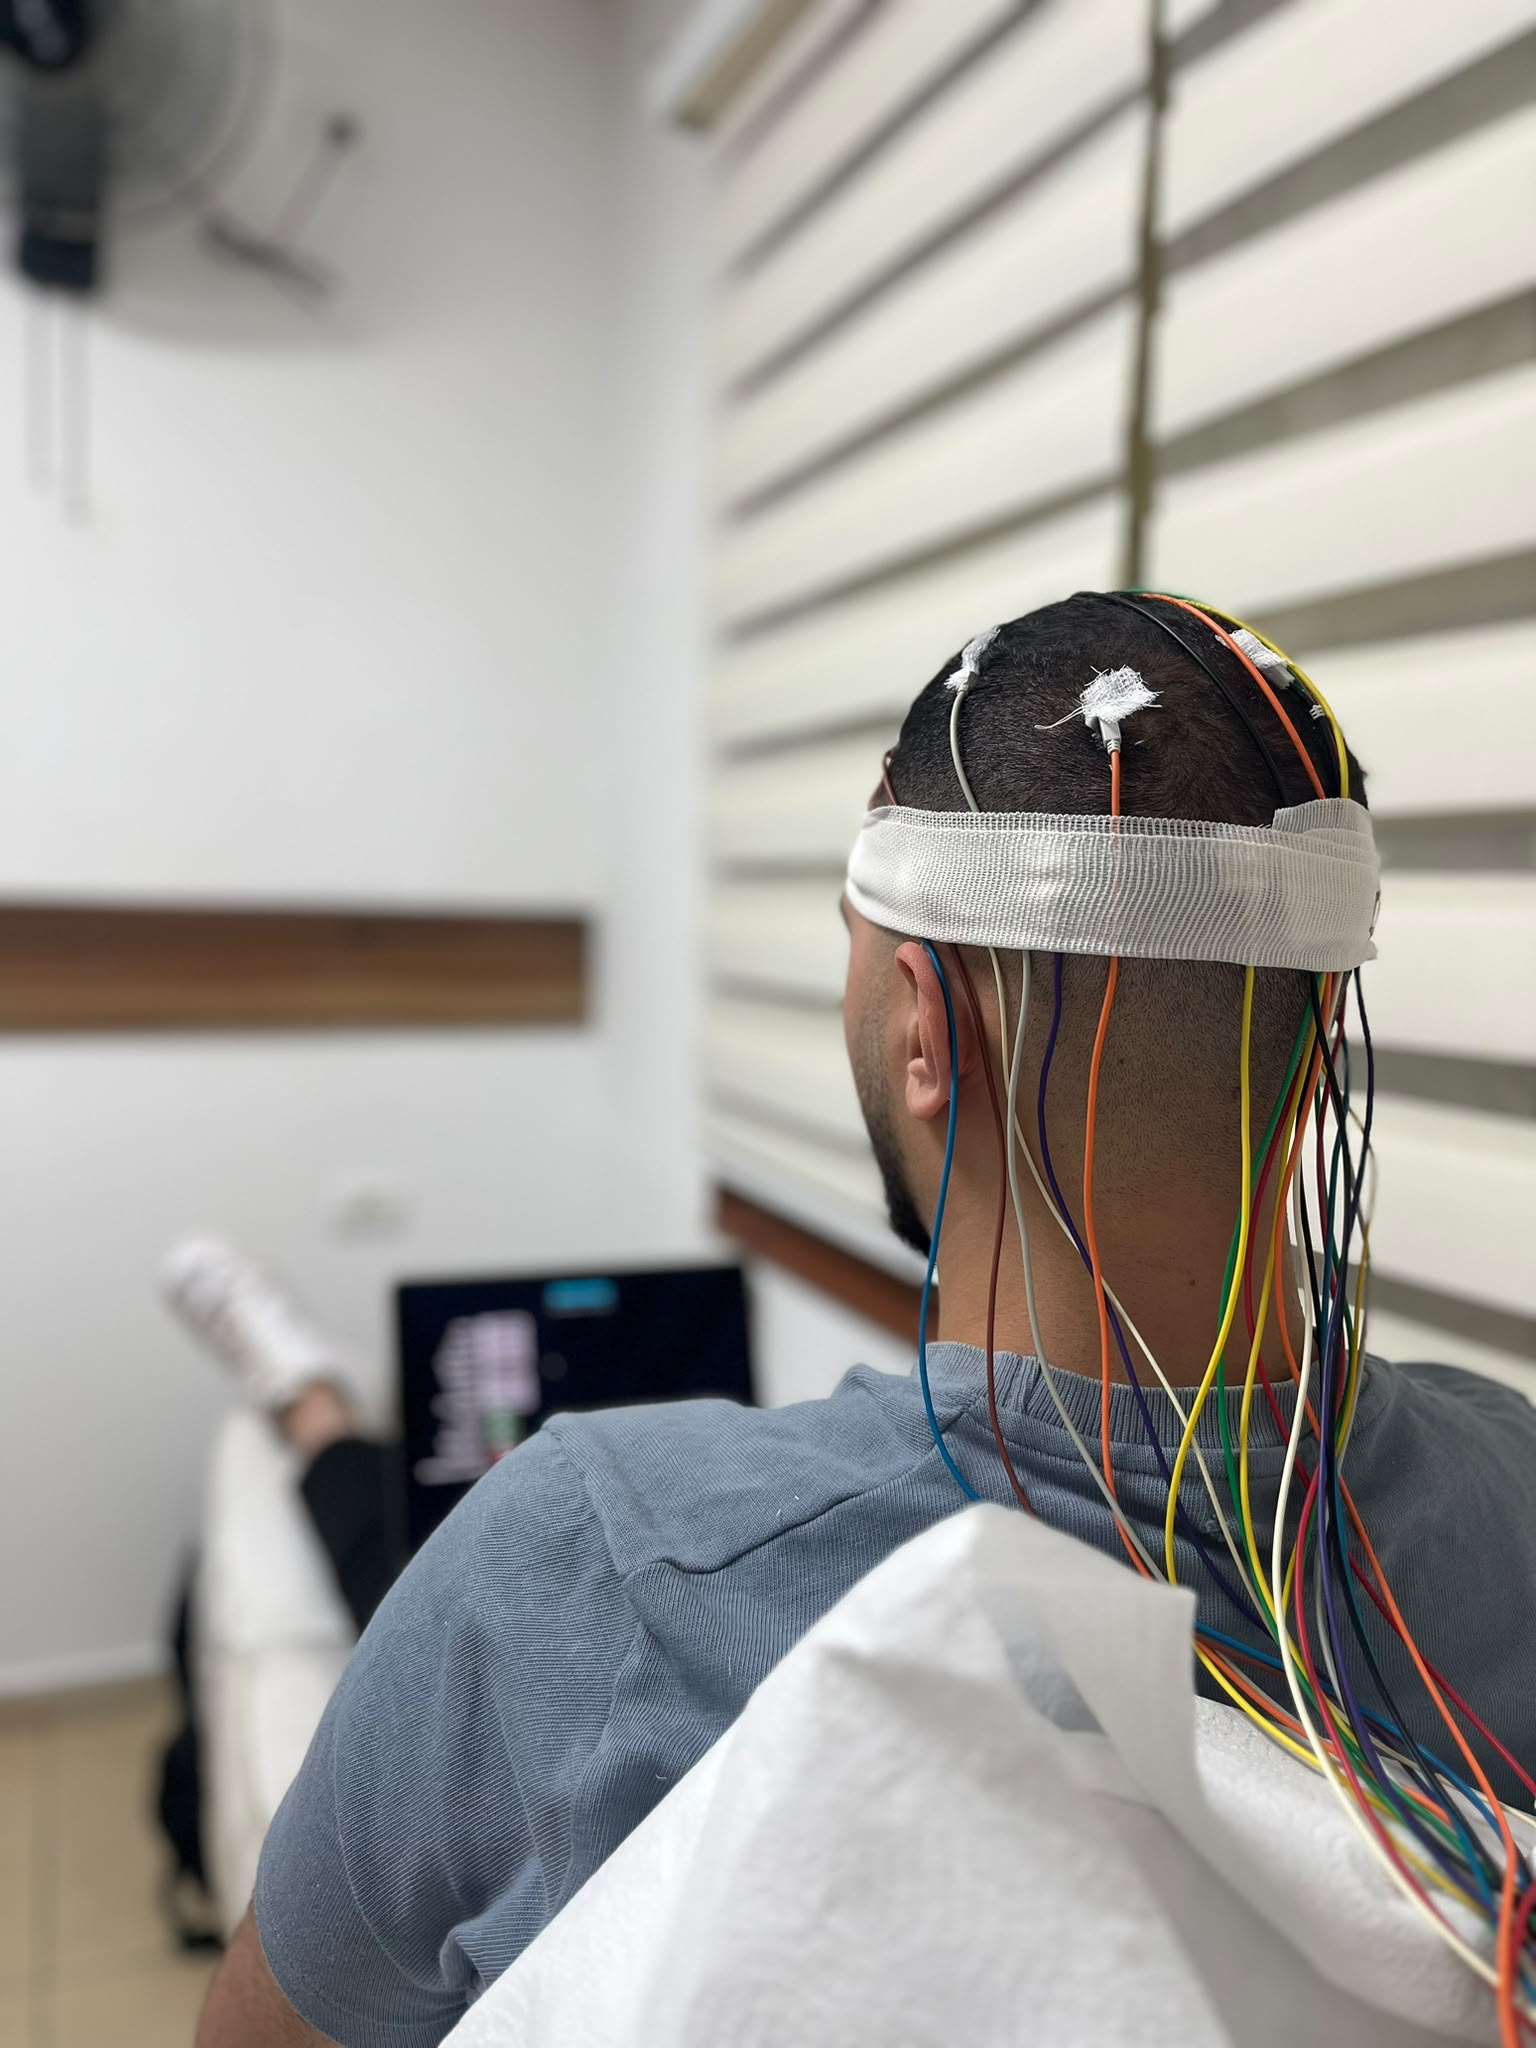
\includegraphics[width=0.75\textwidth]{Assets/subject_eeg_setup}
\caption{Recording environment setup. The subject is seated
comfortably with the 19-channel EEG cap fitted according to
the International 10--20 system. Electrode impedances were
verified below \SI{20}{\kilo\ohm} at all sites before each
session.}
\label{fig:subject_setup}
\end{figure}

\subsection{EEG Setup}

The \acrshort{eeg} cap was fitted according to the International
10--20 electrode placement system, as described in Chapter~3.
Electrode impedances were checked and maintained below
\SI{20}{\kilo\ohm} at all sites before commencing each recording
session. The recording software was configured to capture all 19
channels at \SI{200}{\hertz} and save the output directly to
\acrshort{edf} format (Figure~\ref{fig:eeg_software_in_use}). Each \acrshort{edf} file corresponds to
one continuous recording of a single artifact class (e.g., a
session of repeated double blinks, or a session of repeated jaw
clinches), and each such recording runs 2--5\,minutes, with the
first \SI{40}{\second} cropped during preprocessing to discard
electrode-settling noise (Chapter~7).

\begin{figure}[htbp]
\centering
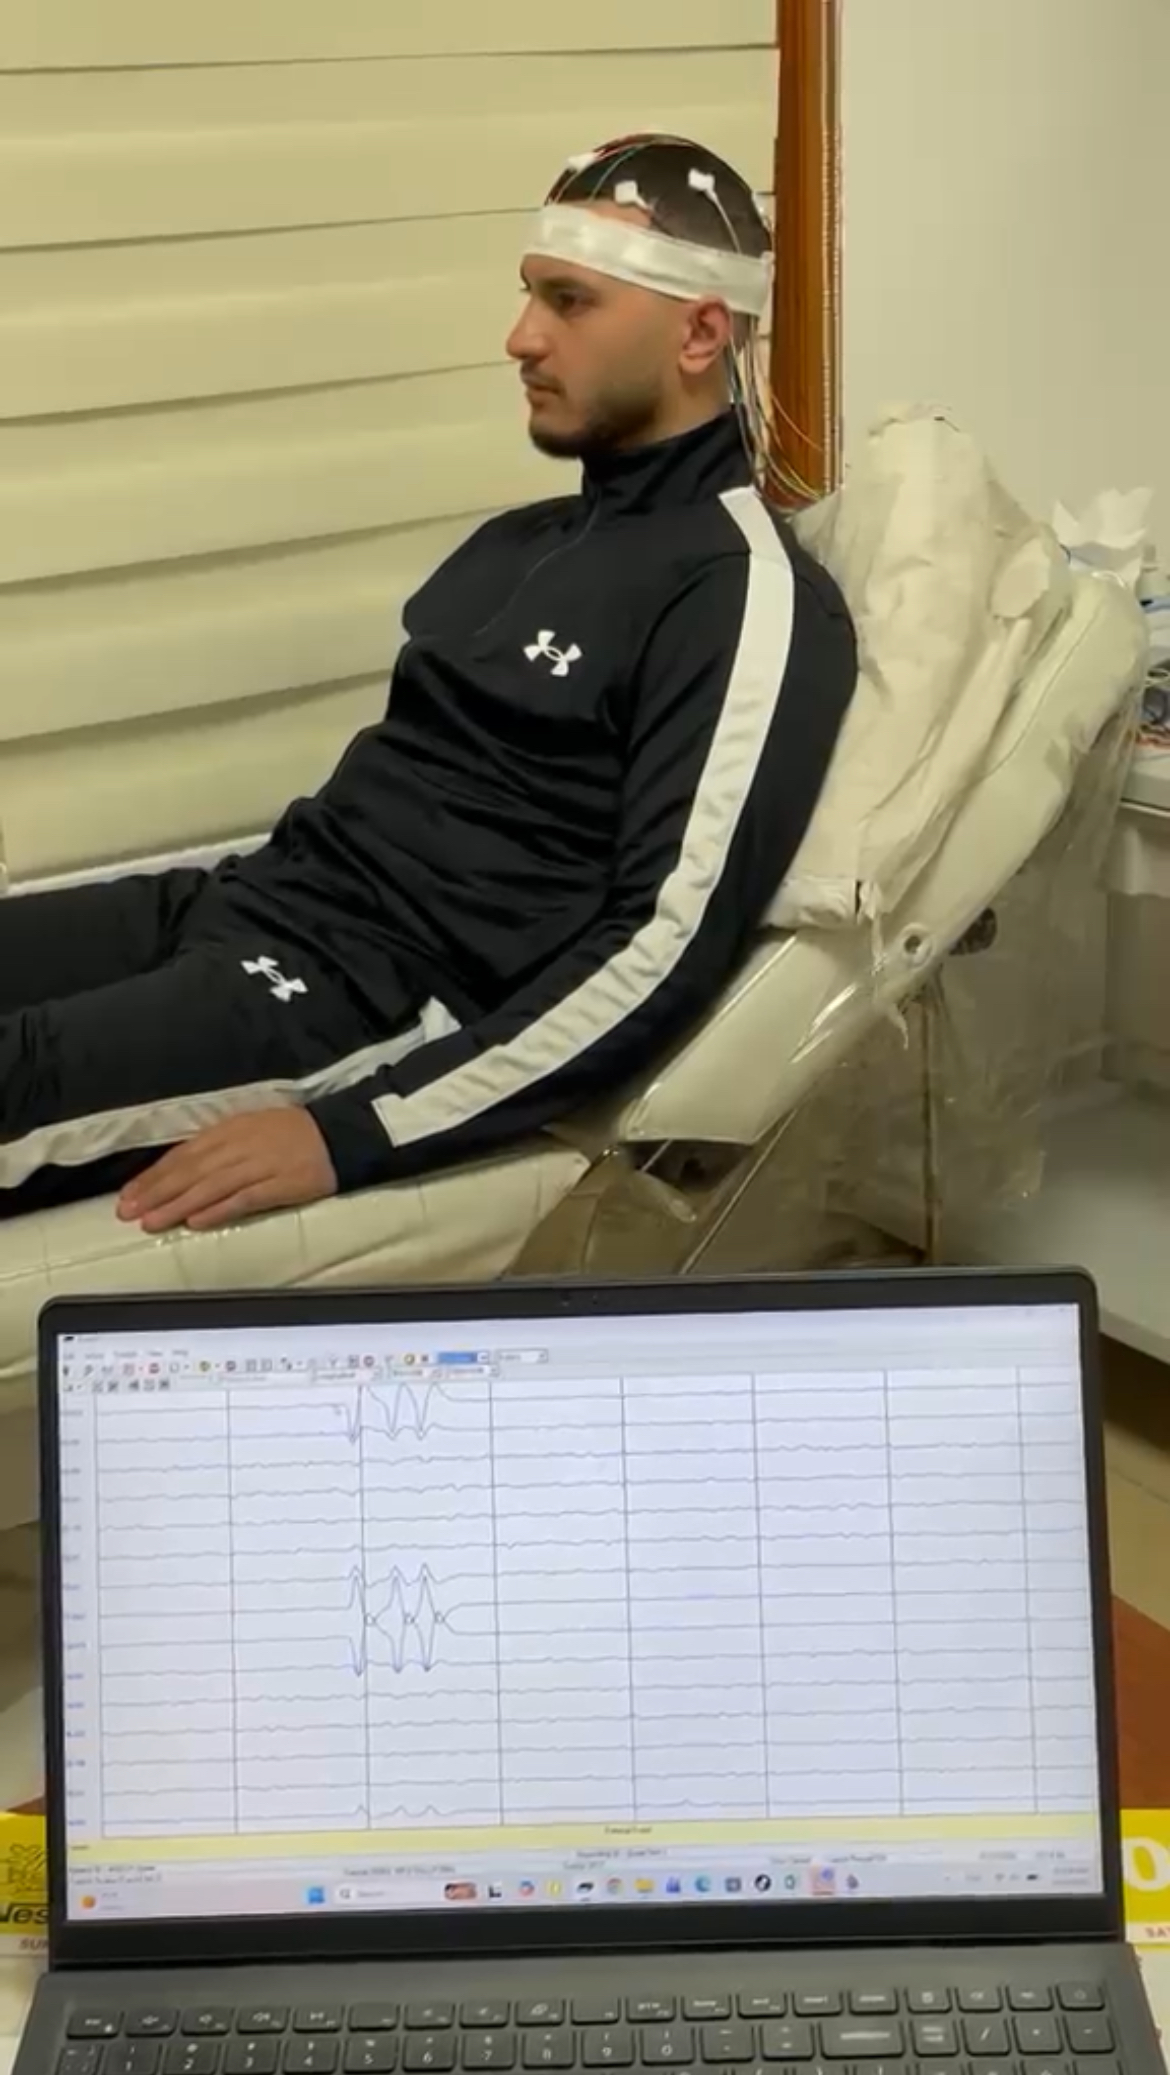
\includegraphics[width=0.7\textwidth]{Assets/eeg_software_in_use}
\caption{A data-collection session in progress. The subject, wearing
the 19-channel cap, sits relaxed while the recording software (laptop,
foreground) displays the live multichannel \acrshort{eeg}; the
large-amplitude deflections visible on the frontal traces correspond
to voluntary artifact events. The stimulus-presentation application
of Section~\ref{sec:dc_protocol} runs alongside to cue the subject and
log trial markers.}
\label{fig:eeg_software_in_use}
\end{figure}

Table~\ref{tab:recording_params} summarises the recording
parameters used across all sessions.

\begin{table}[htbp]
\centering
\caption{EEG recording parameters used in all data collection
sessions.}
\label{tab:recording_params}
\renewcommand{\arraystretch}{1.3}
\begin{tabular}{ll}
\toprule
\textbf{Parameter} & \textbf{Value} \\
\midrule
Number of channels          & 19 \\
Sampling rate               & \SI{200}{\hertz} \\
Output format               & European Data Format (EDF) \\
Electrode impedance         & $<$\SI{20}{\kilo\ohm} \\
Recording duration per file & 2--5 minutes (first 40\,s cropped) \\
Subject posture             & Seated, upright, relaxed \\
Environment                 & Quiet laboratory room \\
Number of sessions          & 3 (Session1, Session2, Session3) \\
Session separation          & $\geq$24 hours (cross-day) \\
\bottomrule
\end{tabular}
\end{table}

%% ----------------------------------------------------------
\section{Session Structure and Recording Protocol}
\label{sec:dc_protocol}
%% ----------------------------------------------------------

\subsection{Session Overview}

Data was collected across \textbf{three} recording sessions
(Session1, Session2, and Session3), each separated by at least
24 hours to introduce cross-session variability and test the
system's ability to generalise across electrode placement
differences, physiological state changes, and impedance
variations between sessions. This cross-day structure is what
later makes the Leave-One-Session-Out (\acrshort{loso})
evaluation protocol possible and meaningful (Chapter~9): each
session can be held out in turn as a genuinely unseen test day,
rather than an artificial split of a single recording.

The data-collection protocol was originally designed around a
broader set of \textbf{nine} target gesture classes --- single,
double, and triple blink; bilateral, left, and right jaw clench;
and bilateral, left, and right bruxism --- to give the widest
possible margin for the classification design to select from.
Over the course of the experimentation described in this and the
following chapters, this set was narrowed twice
(Section~\ref{sec:dc_labels}) down to the five classes that make
up the final, deployed command set: \code{single\_blink},
\code{double\_blink}, \code{clinch}, \code{bruxism\_left}, and
\code{bruxism\_right}.

Each session covered all target artifact classes, with one
\acrshort{edf} recording file per class (or per laterality, for
bruxism and clinch). Within each recording, the subject performed
the target gesture repeatedly under a \textbf{cue-driven protocol}
delivered by a custom stimulus-presentation and marker-logging
application developed for this project
(Figure~\ref{fig:stimulus_setup}). For every trial the application
presents a visual --- and optional audio --- cue naming the gesture,
a fixed action window during which the subject performs it, and a
rest window, following a repeating
CUE\,$\rightarrow$\,GO\,$\rightarrow$\,REST structure
(Section~\ref{sec:dc_trial}). The onset of every trial is written to
a time-stamped marker file that is later aligned against the
\acrshort{edf} recording to label the data. A cue-driven protocol
was chosen because it yields precisely time-locked labels and a
consistent, repeatable trial structure across sessions --- both of
which are prerequisites for the fixed-window epoching and activity
gating described in Chapter~7.

\begin{figure}[htbp]
\centering
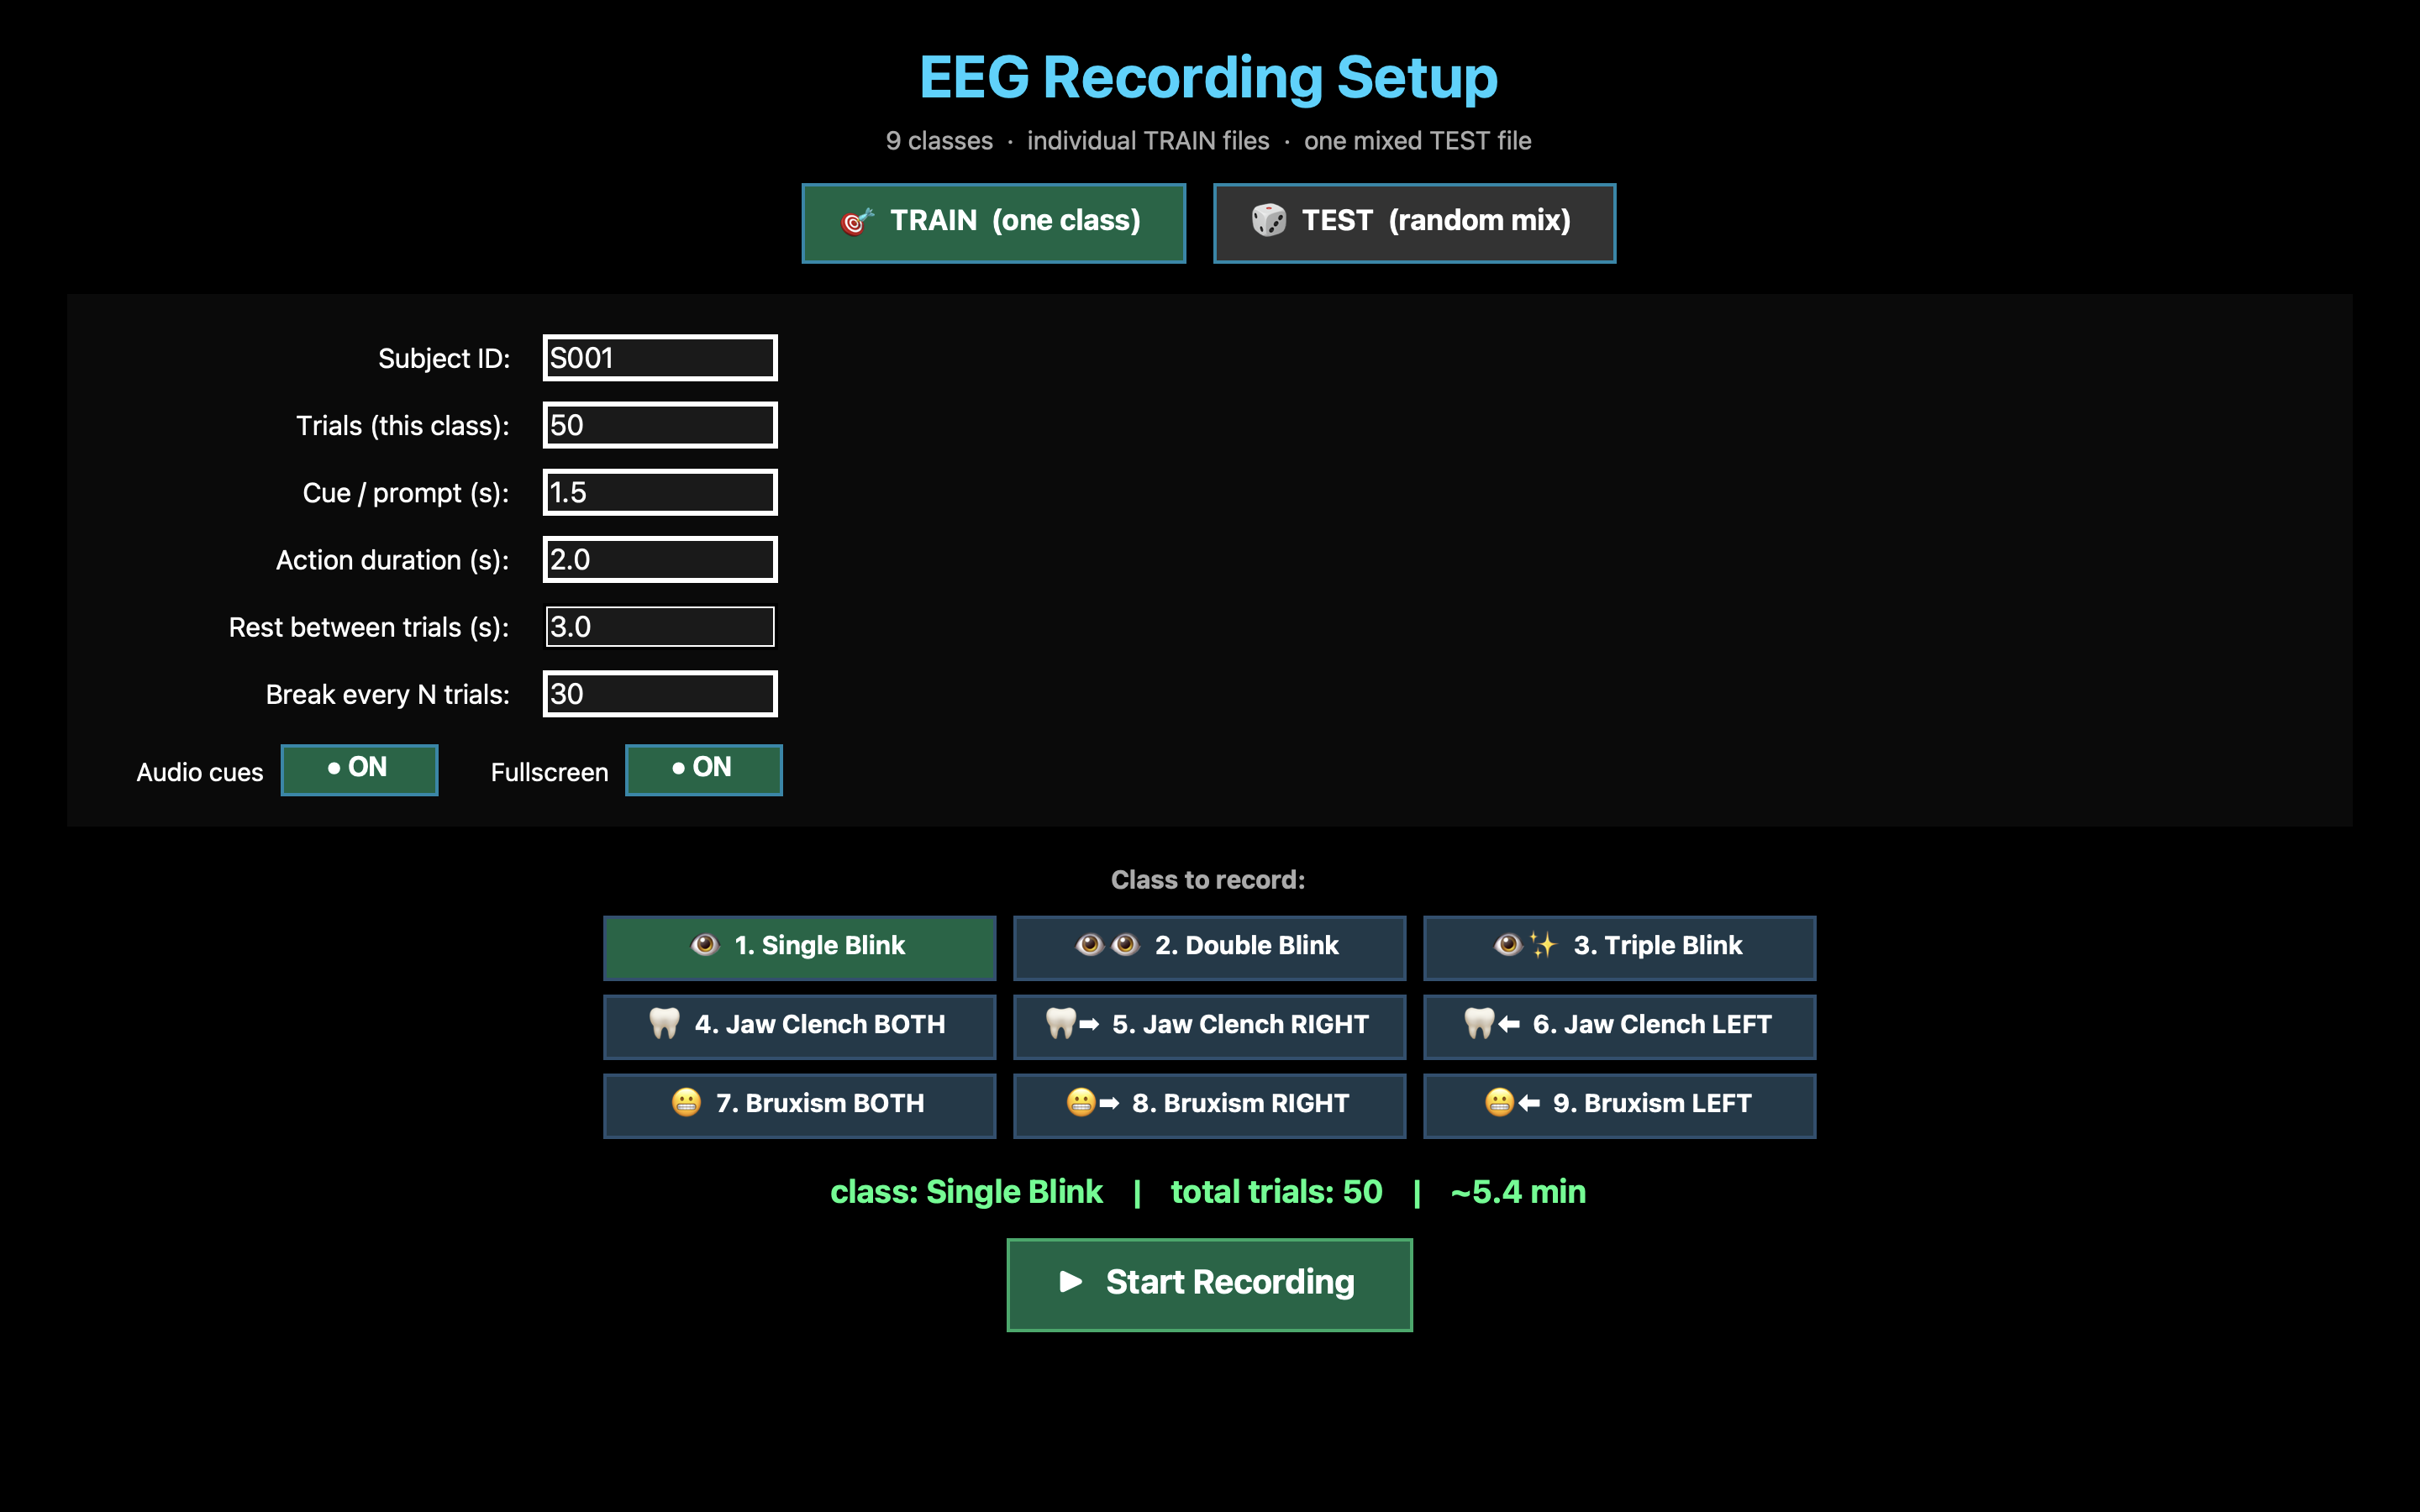
\includegraphics[width=0.90\textwidth]{Assets/stimulus_setup}
\caption{The custom stimulus-presentation and marker-logging
application built for data collection, shown in its session-setup
screen. The operator selects TRAIN mode (record one class
repeatedly, one file per class) or TEST mode (a random mix of all
classes in one file), sets the per-trial timing (cue, action, and
rest durations) and trial count, and chooses one of the nine
originally cued gesture classes --- single, double, and triple
blink; jaw clench (both/right/left); and bruxism (both/right/left)
--- later narrowed to the final five (Section~\ref{sec:dc_labels}).}
\label{fig:stimulus_setup}
\end{figure}

\subsection{Trial Structure Within a Recording}
\label{sec:dc_trial}

Each recording file contains a continuous sequence of gesture
trials interspersed with rest periods, as illustrated in
Figure~\ref{fig:trial_structure}.

\begin{figure}[htbp]
\centering
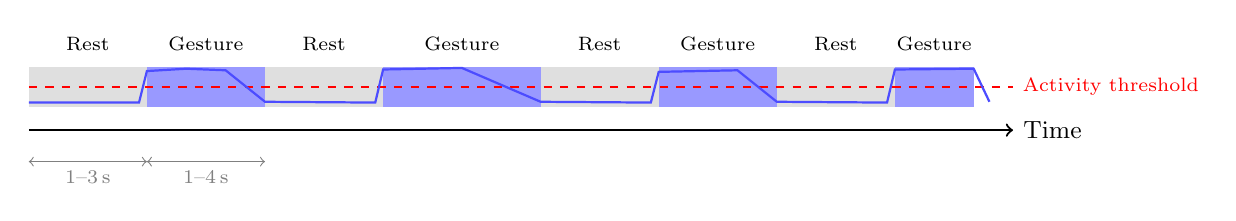
\begin{tikzpicture}[scale=1.0]
    \draw[thick, ->] (0,0) -- (12.5,0) node[right]{\small Time};

    \fill[gray!25] (0,0.3)    rectangle (1.5,0.8);
    \fill[gray!25] (3.0,0.3)  rectangle (4.5,0.8);
    \fill[gray!25] (6.5,0.3)  rectangle (8.0,0.8);
    \fill[gray!25] (9.5,0.3)  rectangle (11.0,0.8);

    \fill[blue!40] (1.5,0.3)  rectangle (3.0,0.8);
    \fill[blue!40] (4.5,0.3)  rectangle (6.5,0.8);
    \fill[blue!40] (8.0,0.3)  rectangle (9.5,0.8);
    \fill[blue!40] (11.0,0.3) rectangle (12.0,0.8);

    \node[font=\scriptsize] at (0.75, 1.1)  {Rest};
    \node[font=\scriptsize] at (2.25, 1.1)  {Gesture};
    \node[font=\scriptsize] at (3.75, 1.1)  {Rest};
    \node[font=\scriptsize] at (5.5,  1.1)  {Gesture};
    \node[font=\scriptsize] at (7.25, 1.1)  {Rest};
    \node[font=\scriptsize] at (8.75, 1.1)  {Gesture};
    \node[font=\scriptsize] at (10.25,1.1)  {Rest};
    \node[font=\scriptsize] at (11.5, 1.1)  {Gesture};

    \draw[<->, gray] (0,-0.4)   -- (1.5,-0.4)
        node[midway, below, font=\scriptsize]{1--3\,s};
    \draw[<->, gray] (1.5,-0.4) -- (3.0,-0.4)
        node[midway, below, font=\scriptsize]{1--4\,s};

    \draw[red, dashed, thick] (0,0.55) -- (12.5,0.55);
    \node[red, font=\scriptsize, right] at (12.5,0.55)
        {Activity threshold};

    \draw[blue!70, thick]
        (0,0.35)   -- (1.4,0.35) -- (1.5,0.75) -- (2.0,0.78)
        -- (2.5,0.76) -- (3.0,0.36) -- (4.4,0.35) -- (4.5,0.77)
        -- (5.5,0.79) -- (6.5,0.36) -- (7.9,0.35) -- (8.0,0.74)
        -- (9.0,0.76) -- (9.5,0.36) -- (10.9,0.35) -- (11.0,0.77)
        -- (12.0,0.78) -- (12.2,0.36);
\end{tikzpicture}
\caption{Schematic of the trial structure within a single EDF
recording. Active gesture periods (blue) alternate with rest
periods (gray). The activity gate threshold (red dashed line)
is used during preprocessing to retain only epochs where the
RMS energy exceeds the threshold, discarding rest-period epochs
that carry the gesture class label but contain no gesture signal
(Chapter~7).}
\label{fig:trial_structure}
\end{figure}

\subsection{Recording Files and Folder Organisation}

\begin{figure}[htbp]
\centering
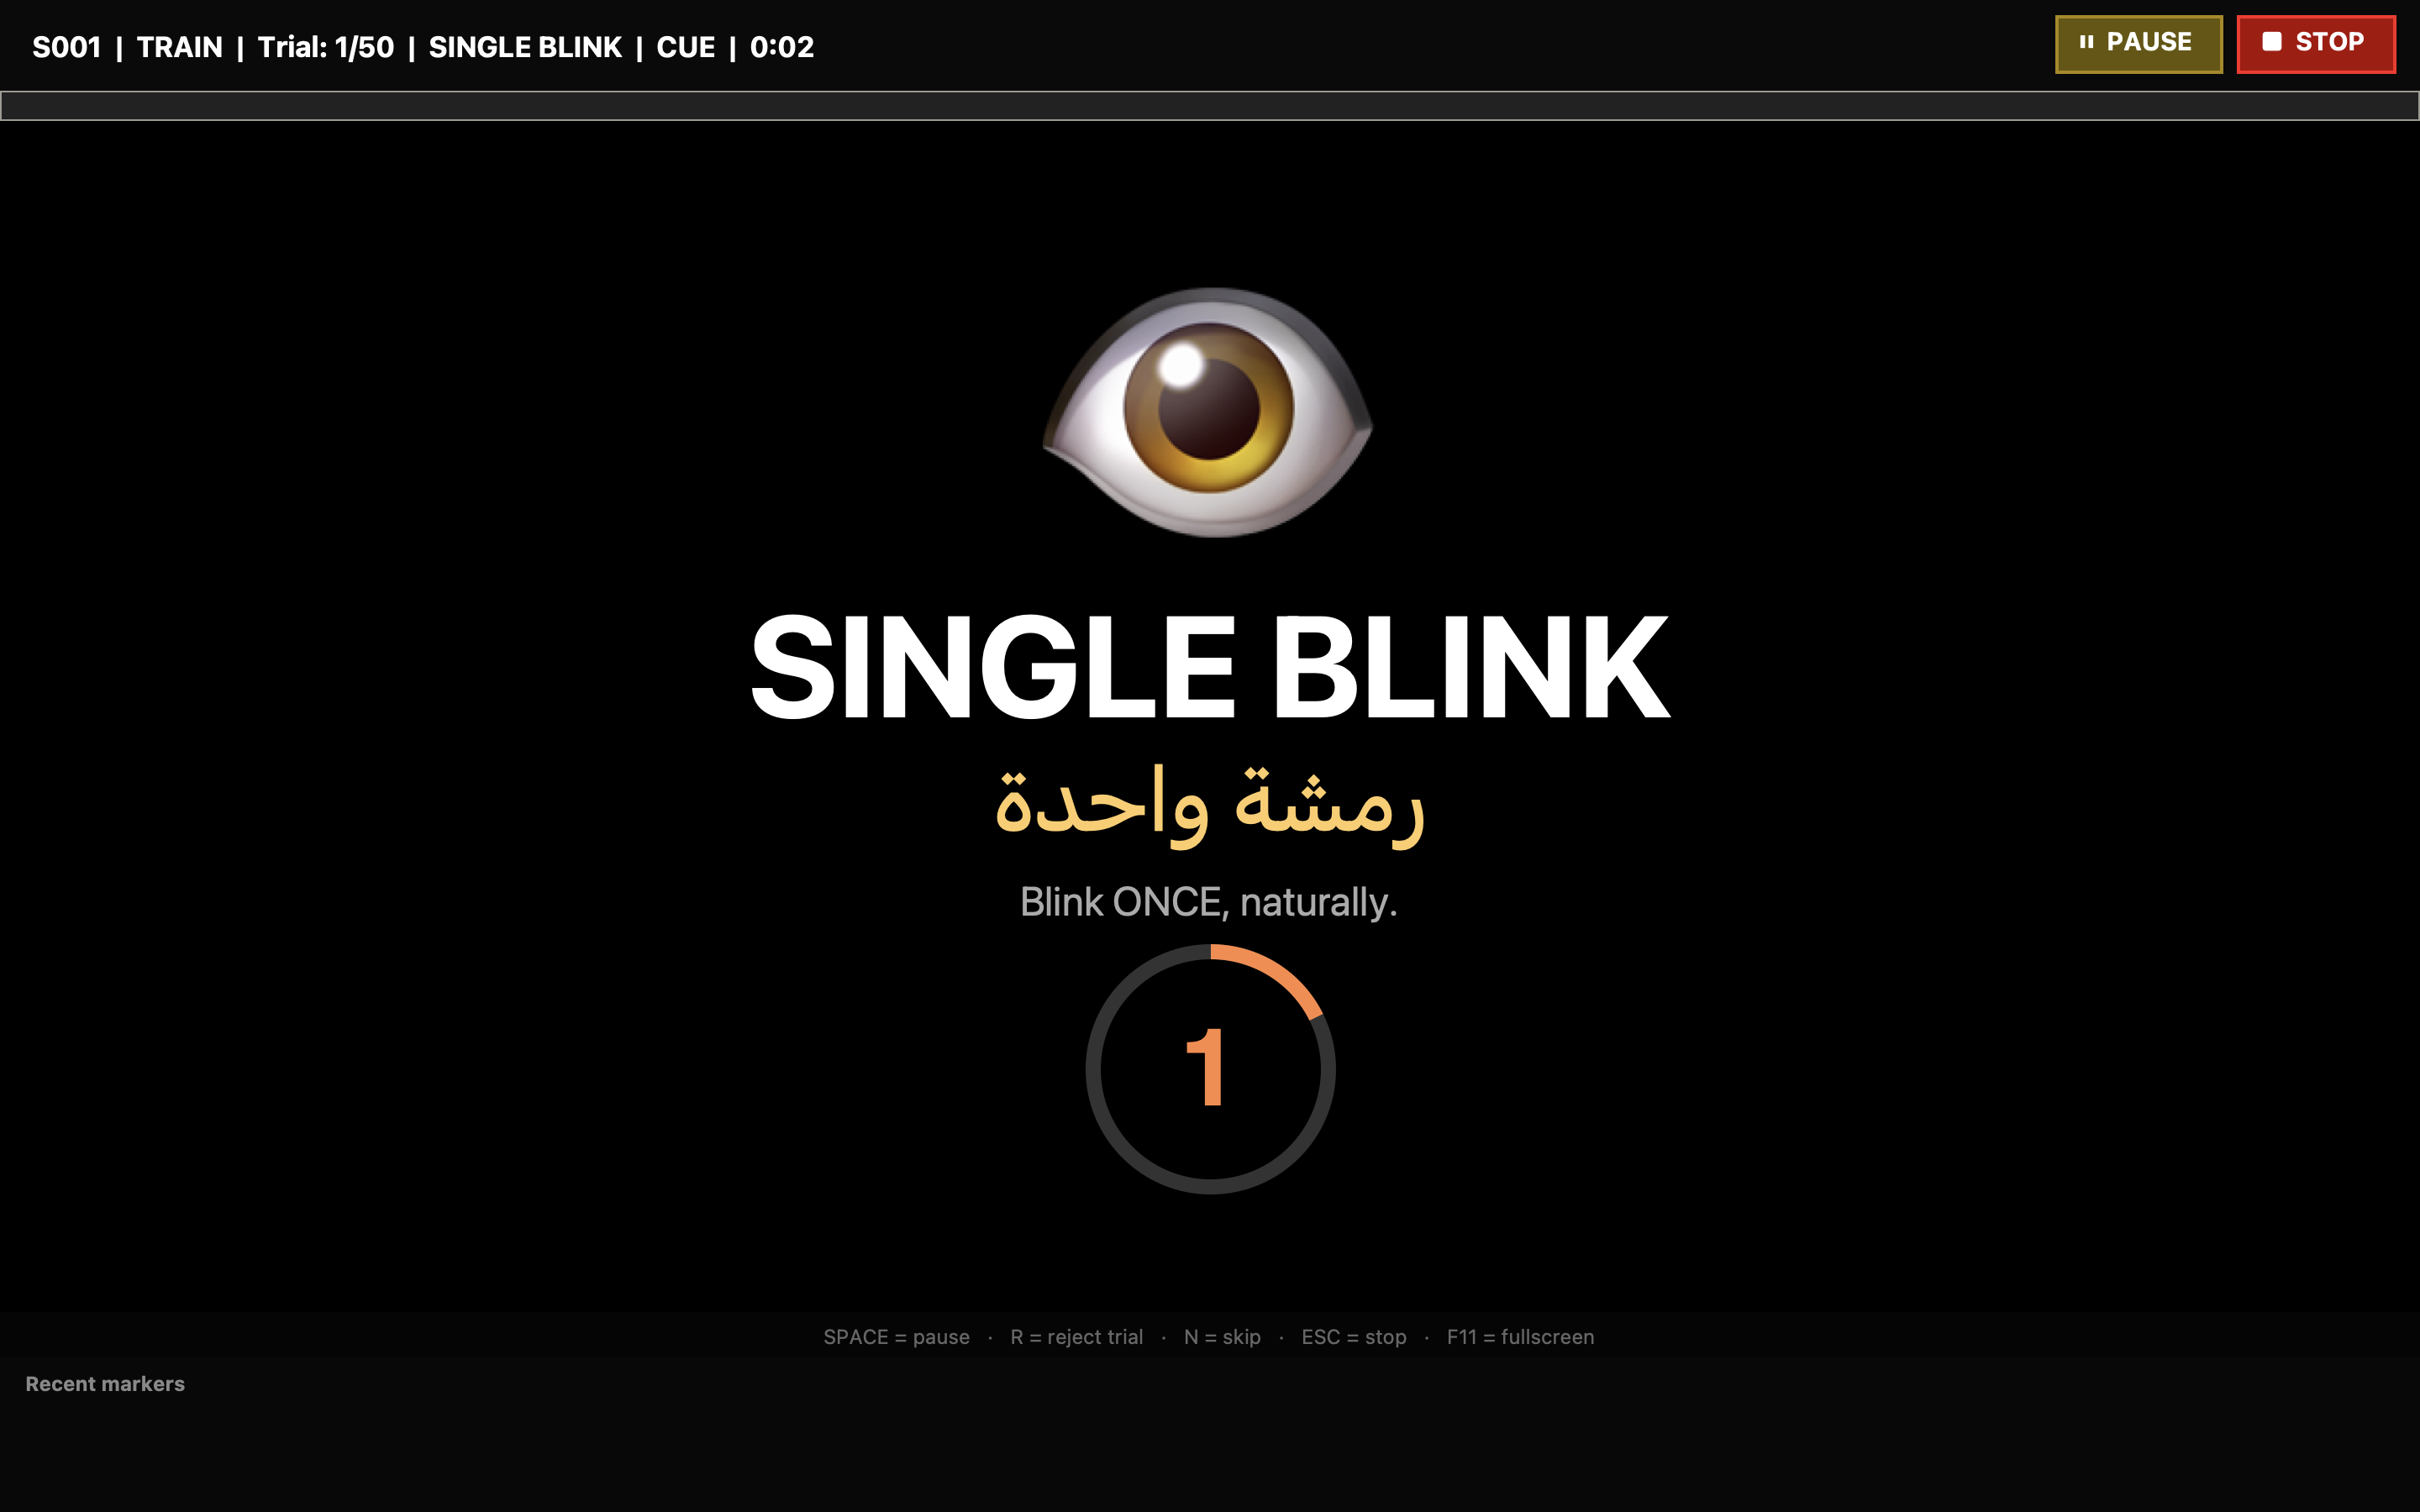
\includegraphics[width=0.90\textwidth]{Assets/stimulus_cue_single_blink}
\caption{A single trial cue as presented to the subject by the
stimulus application (here the \code{single\_blink} class, CUE
phase). Each trial shows the gesture name, a bilingual instruction
and icon, and a countdown ring that transitions the subject from
CUE to the GO (action) window; a running log of accepted/rejected
trial markers is kept at the foot of the screen. This is the
cue-driven mechanism referenced in Section~\ref{sec:dc_protocol}.}
\label{fig:stimulus_cue}
\end{figure}

Each recording session is organised into three sub-folders
corresponding to the three artifact modality groups: Blink,
Bruxissem, and Clinch. \textbf{Session1} and \textbf{Session2}
share one file-naming convention; \textbf{Session3} was recorded
using a second, differently-named convention, which the loader
must reconcile (Section~\ref{sec:dc_structure}). Each session
folder contains recordings for the full nine-class protocol
described above, but the data loader used for the final system
(\code{loader.discover\_recordings}) selects exactly \textbf{one
recording per session per final class}, giving
\textbf{15 \acrshort{edf} recordings} in total (3 sessions
$\times$ 5 classes) that feed the reported dataset statistics in
Section~\ref{sec:dc_stats}:

\begin{itemize}[leftmargin=*]
    \item \textbf{Blink/} --- up to three \acrshort{edf} files
    per session, one per blink type (\code{BLINK01.edf} for
    single blinks, \code{BLINK02.edf} for double blinks,
    \code{BLINK03.edf} for triple/multi-blink bursts). Only
    \code{BLINK01} and \code{BLINK02} are selected by the loader
    for the final 5-class dataset; \code{BLINK03} is present on
    disk but excluded (Section~\ref{sec:dc_labels}).

    \item \textbf{Bruxissem/} --- in Session1/Session2, files
    named \code{LEFT.edf} and \code{RIGHT.edf}, plus a bilateral
    recording. In Session3, the equivalent files are named
    \code{BRUXESLEFT}, \code{BRUXESRIGHT}, and
    \code{BRUXESDOUBLE}. Only the left and right recordings are
    selected; the bilateral (``double'') recording is present on
    disk but excluded. Note: the folder name ``Bruxissem'' is
    retained from the original recording software output and is
    handled as-is by the data loader.

    \item \textbf{Clinch/} --- in Session1/Session2, organised
    into sub-folders (\code{Bilateral}, \code{Bileteral} --- note
    the spelling variant, a folder-naming typo that caused a
    silent data-loss bug during earlier development, described in
    Section~\ref{sec:dc_bug}). In Session3, the equivalent files
    use a different naming convention (\code{GLENCHLEFT},
    \code{GLENCHRIGHT}, \code{GLENCHDOUBLE}). Exactly one clinch
    recording per session is selected for the final dataset.
\end{itemize}

The bilateral recordings excluded above (\code{BRUXESDOUBLE},
\code{GLENCHDOUBLE}, and their Session1/2 equivalents) deserve a
specific note: bilateral bruxism had, during an earlier analysis
pass, been mislabelled and folded into the \code{clinch} class,
which silently corrupted that class's decision boundary. Once
diagnosed, bilateral bruxism was excluded from training entirely
rather than re-labelled, as part of the taxonomy simplification
described in Section~\ref{sec:dc_labels}. It is documented here
as a class that was recorded but deliberately not used in the
final 5-class scheme.

%% ----------------------------------------------------------
\section{Artifact Gesture Protocols}
\label{sec:dc_gestures}
%% ----------------------------------------------------------

This section provides detailed descriptions of each of the five
voluntary artifact gestures retained in the final classification
scheme, including the physiological mechanism by which each
gesture produces a distinctive \acrshort{eeg} signal, the
recording instructions given to the subject, and the
characteristic signal morphology at the relevant electrode
sites. The gesture-to-command mapping used throughout the rest
of this report is: single blink $\rightarrow$ \code{O} (open
hand), double blink $\rightarrow$ \code{S} (start/confirm), jaw
clinch $\rightarrow$ \code{C} (close hand), left bruxism
$\rightarrow$ \code{L} (rotate left), right bruxism
$\rightarrow$ \code{R} (rotate right).

\subsection{Single Blink (Class: \texttt{single\_blink})}
\label{sec:dc_single_blink}

\textbf{Physiological mechanism:} A voluntary eye blink involves
a rapid closure and reopening of the eyelid driven by the
orbicularis oculi muscle, lasting approximately 150--400\,ms.
The movement of the eyelid over the cornea sweeps the
corneoretinal potential across the frontal scalp, inducing a
large-amplitude deflection primarily at Fp1 and Fp2. The signal
waveform is characterised by a single sharp peak with amplitude
approximately 50--350\,\si{\micro\volt}, followed by a slower
return to baseline.

\textbf{Recording instruction:} The subject performed one
deliberate, complete eye blink, then waited 2--4\,seconds in a
relaxed eyes-open state before performing the next blink.

\textbf{Key electrodes:} Fp1, Fp2 (primary); F3, F4, F7, F8
(secondary, smaller amplitude).

\begin{figure}[htbp]
\centering
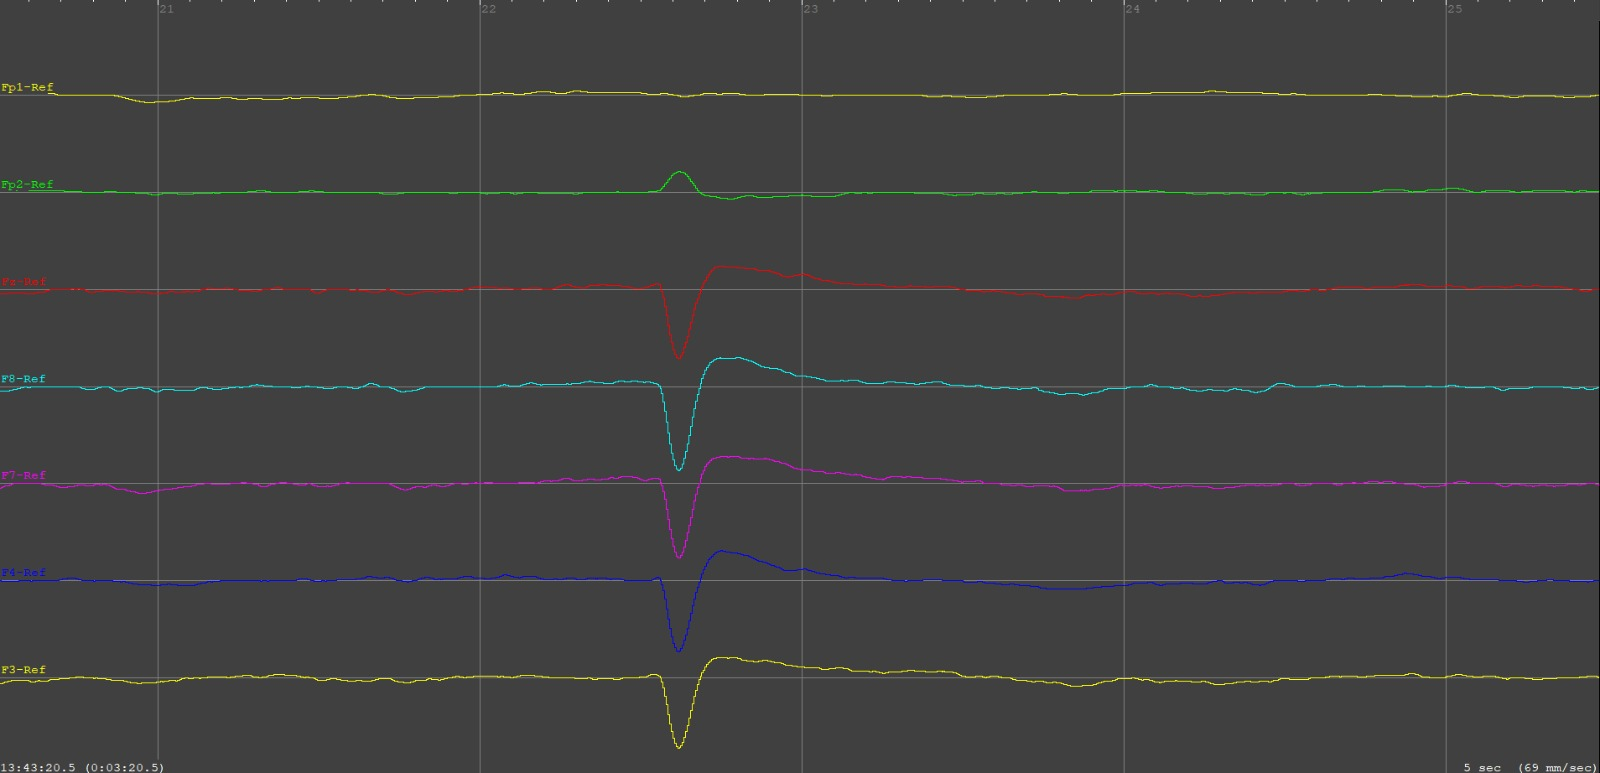
\includegraphics[width=0.90\textwidth]{Assets/signal_single_blink}
\caption{EEG signal at Fp1 and Fp2 during a voluntary single
blink. The characteristic single large-amplitude peak is
clearly visible at both frontal electrodes, with rapid onset
and slower return to baseline.}
\label{fig:signal_single_blink}
\end{figure}

\textbf{Data quality issue --- single-blink contamination
(critical finding):} A detailed diagnostic pass, performed while
building the event-locked blink detector for Chapter~9, revealed
that the \code{BLINK01} (``single blink'') recordings were not
as pure as their label implied. Automated blink counting showed
an average of 2.60 detected blinks per nominal ``single blink''
trial, with only about 39\% of trials containing a genuinely
isolated blink; roughly \textbf{45\% of ``single blink'' trials
actually contained a cluster of three or more blinks within
about one second} of each other, i.e., the subject had
inadvertently produced a multi-blink burst rather than a single
clean blink. By contrast, the same diagnostic showed the
\code{double\_blink} and \code{triple\_blink} recordings were
largely clean (an average of 2.07 and 3.08 detected blinks per
trial, respectively).

This is a data-quality property of the recorded \code{single\_blink}
class itself, not a bug in the labelling pipeline: the marker
labels are correct (each trial is drawn from the file the subject
was told to record as ``single blink''), but a meaningful fraction
of what the subject actually produced during those trials was
physically closer to a double- or triple-blink burst. Because one
class's recordings contain instances that look like another
class, no purely event-counting approach can cleanly separate
\code{single\_blink} from \code{double\_blink} using this data ---
four independent counting-based methods were tried and rejected
for exactly this reason (Chapter~9). This discovery directly
motivated the shift to Dynamic Time Warping (\acrshort{dtw})
shape-matching for blink sub-classification, which compares
waveform morphology rather than counting discrete events, and is
described in full in Chapter~9.

\subsection{Double Blink (Class: \texttt{double\_blink})}

\textbf{Physiological mechanism:} A double blink consists of
two complete blink cycles performed in rapid succession, with
an inter-blink interval of approximately 200--400\,ms. The
resulting \acrshort{eeg} signal at Fp1/Fp2 contains two
identifiable deflection peaks within roughly a
600--900\,ms window, distinguishing it from a single, isolated
blink.

\textbf{Recording instruction:} The subject performed two rapid
blinks in quick succession (``blink-blink''), then waited
3--5\,seconds before the next double blink.

\textbf{Key electrodes:} Fp1, Fp2 (two peaks within window).

\textbf{Classification challenge:} Together with
\code{single\_blink}, this is the harder half of the taxonomy:
in the final \acrshort{dtw}-hybrid architecture (Chapter~9) it
achieves an \acrshort{loso} F1 of 0.806, the lowest of the five
final classes, reflecting both the natural timing variability of
the inter-blink interval and the residual effect of the
contamination described in Section~\ref{sec:dc_single_blink}.

\begin{figure}[htbp]
\centering
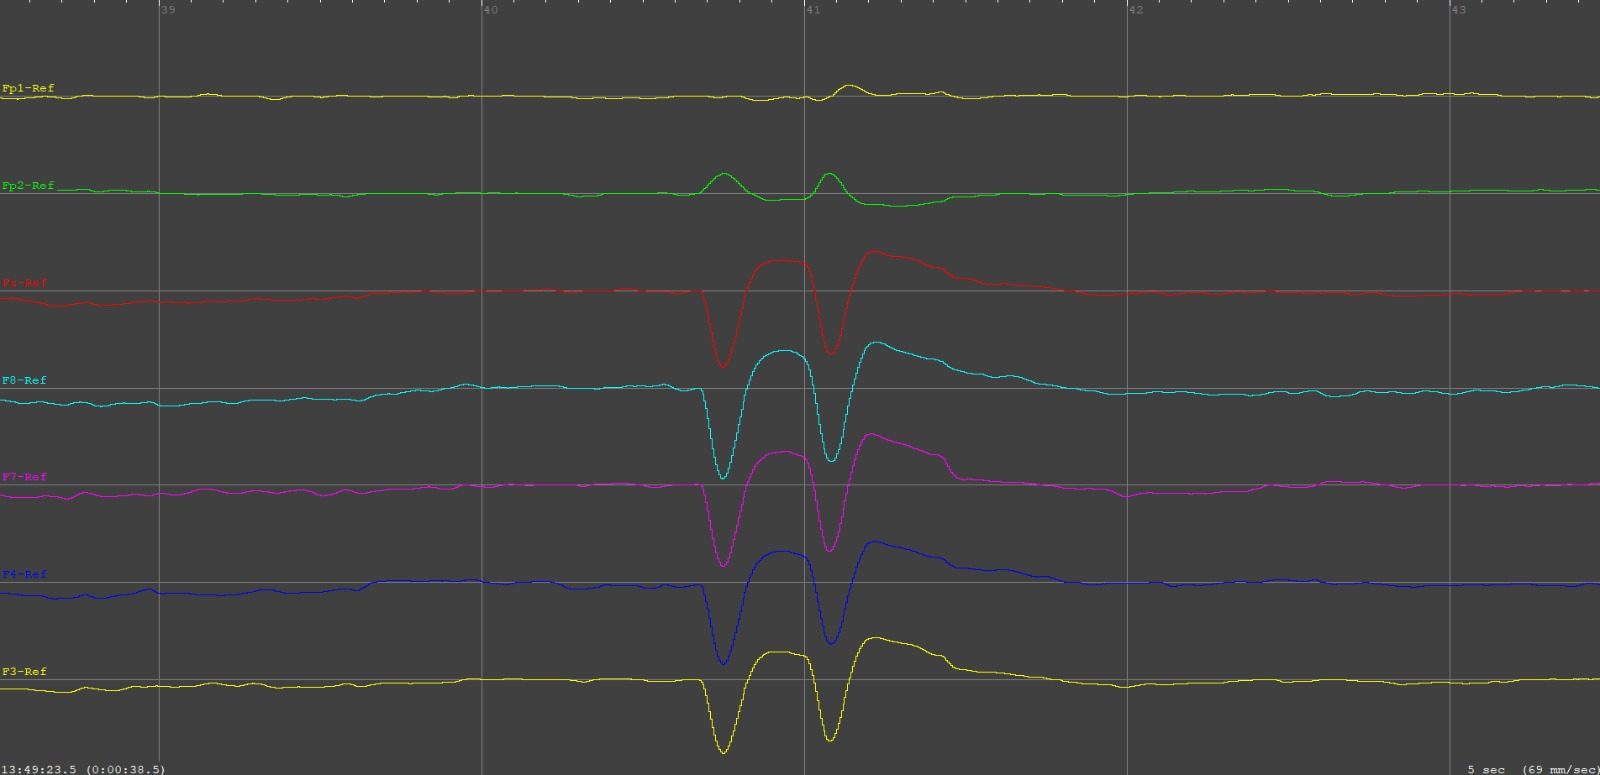
\includegraphics[width=0.90\textwidth]{Assets/signal_double_blink}
\caption{EEG signal at Fp1 and Fp2 during a voluntary double
blink. Two distinct amplitude peaks are visible within the
epoch window, separated by an inter-blink interval of
approximately 200--400\,ms.}
\label{fig:signal_double_blink}
\end{figure}

\subsection{Jaw Clinch (Class: \texttt{clinch})}

\textbf{Physiological mechanism:} A jaw clinch involves a
sustained, forceful bilateral contraction of the masseter and
temporalis muscles, as in biting down hard. The muscle
contraction produces a broadband \acrshort{emg} burst
(30--200\,Hz) that contaminates both temporal channels (T3, T4)
simultaneously with high-amplitude signals (commonly
80--1000\,\si{\micro\volt} at the electrode after broadband
filtering). The bilateral symmetry of the clinch --- roughly
equal activation of T3 and T4 --- distinguishes it from bruxism,
which is lateralised.

\textbf{Recording instruction:} The subject performed a firm
jaw clinch lasting approximately 1--2\,seconds, then relaxed
and waited 3--4\,seconds before the next clinch. Clinch is
consistently the highest-epoch-count class across all three
sessions, owing to the ease and comfort of performing sustained
clinches compared with the shorter, more effortful bruxism and
blink gestures.

\textbf{Key electrodes:} T3 and T4 (bilateral, approximately
equal amplitude); T5, T6 (secondary).

\textbf{Loader bug and its impact:} Section~\ref{sec:dc_bug}
describes a critical data loader bug that caused a portion of
clinch data to be silently discarded during initial training
runs, due to a folder-naming typo.

\begin{figure}[htbp]
\centering
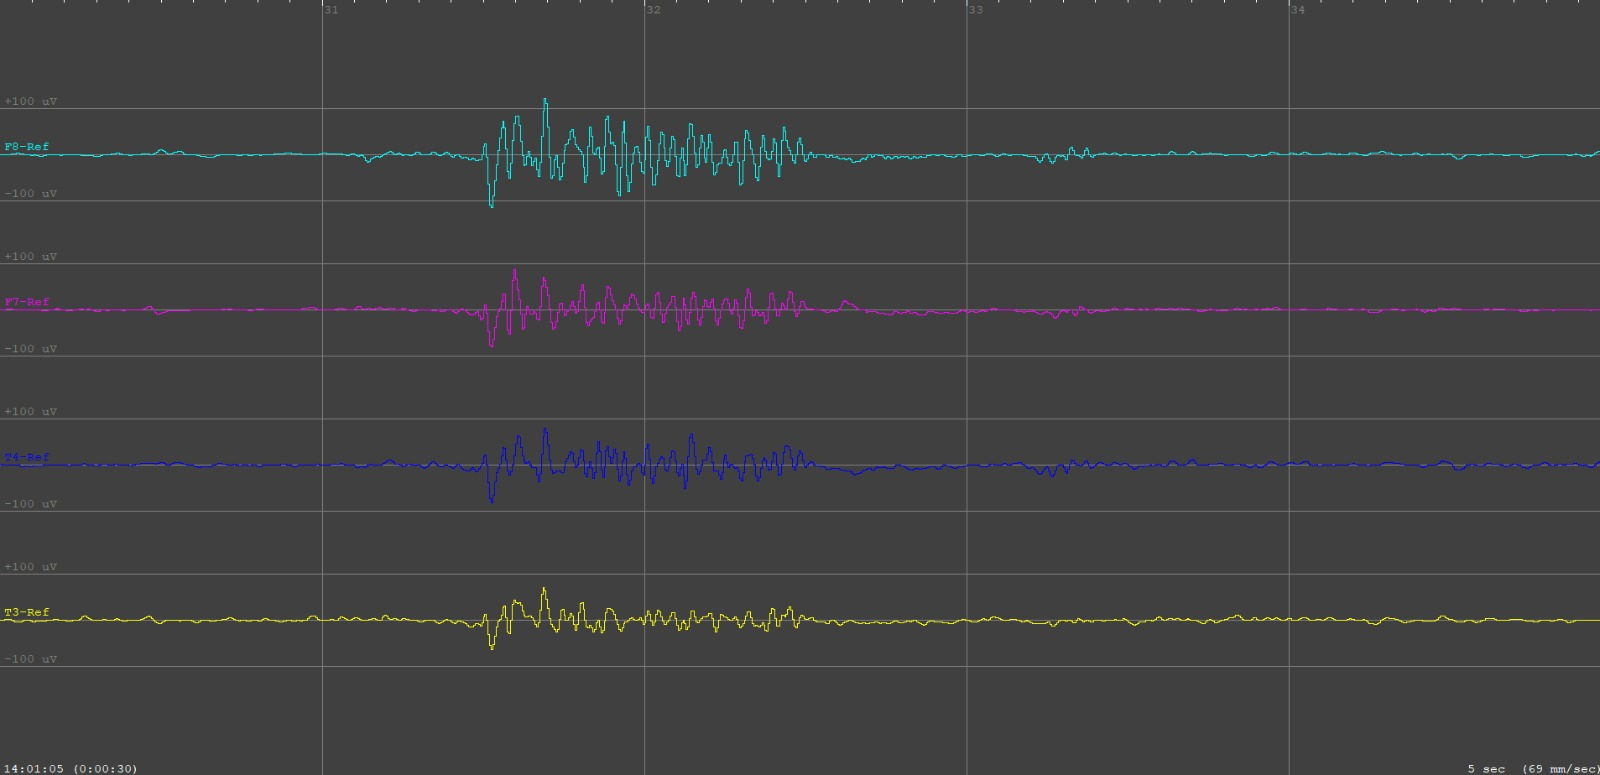
\includegraphics[width=0.90\textwidth]{Assets/signal_clinch}
\caption{EEG signal at T3 and T4 during a voluntary jaw clinch.
Both temporal channels show simultaneous large-amplitude
broadband EMG bursts with approximately equal amplitude
(bilateral symmetry), clearly distinguishable from the resting
baseline before and after the clinch.}
\label{fig:signal_clinch}
\end{figure}

\subsection{Left Bruxism (Class: \texttt{bruxism\_left})}

\textbf{Physiological mechanism:} Bruxism refers to lateral jaw
grinding movements. Left bruxism involves grinding the lower jaw
to the left side relative to the upper jaw, producing preferential
activation of the left temporalis muscle. This lateralised
contraction is captured as a higher-amplitude \acrshort{emg}
signal at T3 (left temporal) compared to T4 (right temporal).

\textbf{Recording instruction:} The subject performed a
deliberate left-directed grinding motion lasting approximately
1\,second, then relaxed and waited 3--5\,seconds before the
next repetition. The subject was instructed to make the motion
feel distinct from a simple clinch by emphasising the leftward
jaw displacement.

\textbf{Key electrodes:} T3 $>$ T4 (T3 dominant); normalised
asymmetry index $(T4 - T3)/(T4 + T3) < 0$.

\textbf{Classification outcome:} Of the five final classes,
\code{bruxism\_left} is the best-classified, reaching an
\acrshort{loso} F1 of 0.984 in the final Riemannian-geometry
muscle branch (Chapter~9) --- its lateral covariance structure
survives cross-session amplitude drift far better than the
amplitude-based features tried earlier in the project.

\begin{figure}[htbp]
\centering
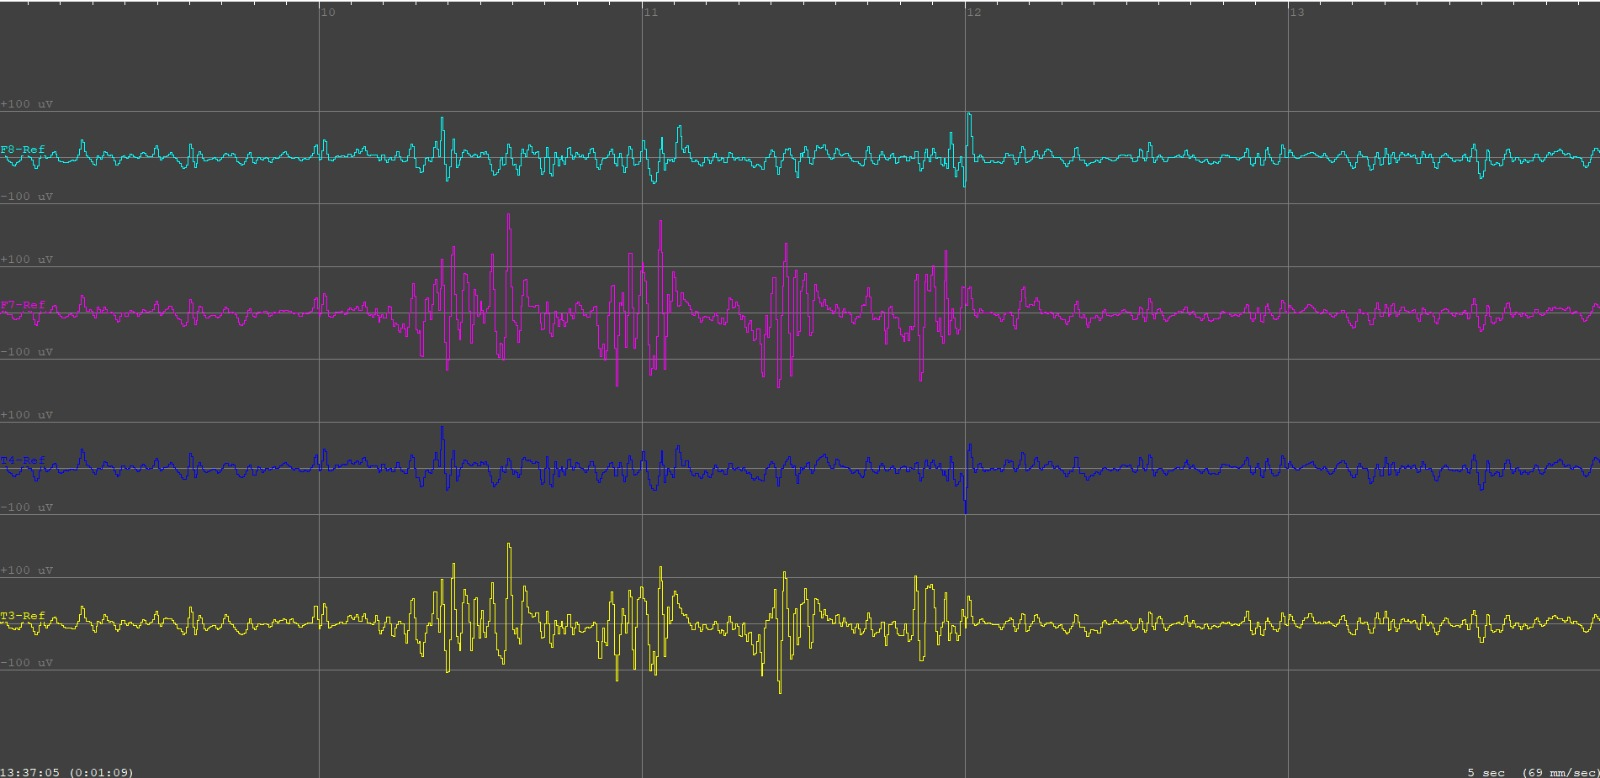
\includegraphics[width=0.90\textwidth]{Assets/signal_bruxism_l}
\caption{EEG signal at T3 and T4 during voluntary \textbf{left
bruxism}. T3 (left temporal) shows clearly higher amplitude
than T4 (right temporal), reflecting preferential activation
of the left temporalis muscle. The normalised asymmetry index
$\mathcal{A}_{T3,T4} < 0$ for this class.}
\label{fig:signal_bruxism_left}
\end{figure}

\subsection{Right Bruxism (Class: \texttt{bruxism\_right})}

\textbf{Physiological mechanism:} Right bruxism involves
grinding the lower jaw to the right side, producing preferential
activation of the right temporalis muscle, captured as a
higher-amplitude signal at T4 (right temporal) compared to T3.

\textbf{Recording instruction:} The subject performed a
deliberate right-directed grinding motion lasting approximately
1\,second, then relaxed and waited 3--5\,seconds before the
next repetition.

\textbf{Key electrodes:} T4 $>$ T3 (T4 dominant); normalised
asymmetry index $(T4 - T3)/(T4 + T3) > 0$.

\textbf{Classification outcome:} \code{bruxism\_right} reaches
an \acrshort{loso} F1 of 0.983, essentially matching
\code{bruxism\_left} and confirming that the Riemannian
covariance approach treats both lateralities symmetrically well
(Chapter~9).

\begin{figure}[htbp]
\centering
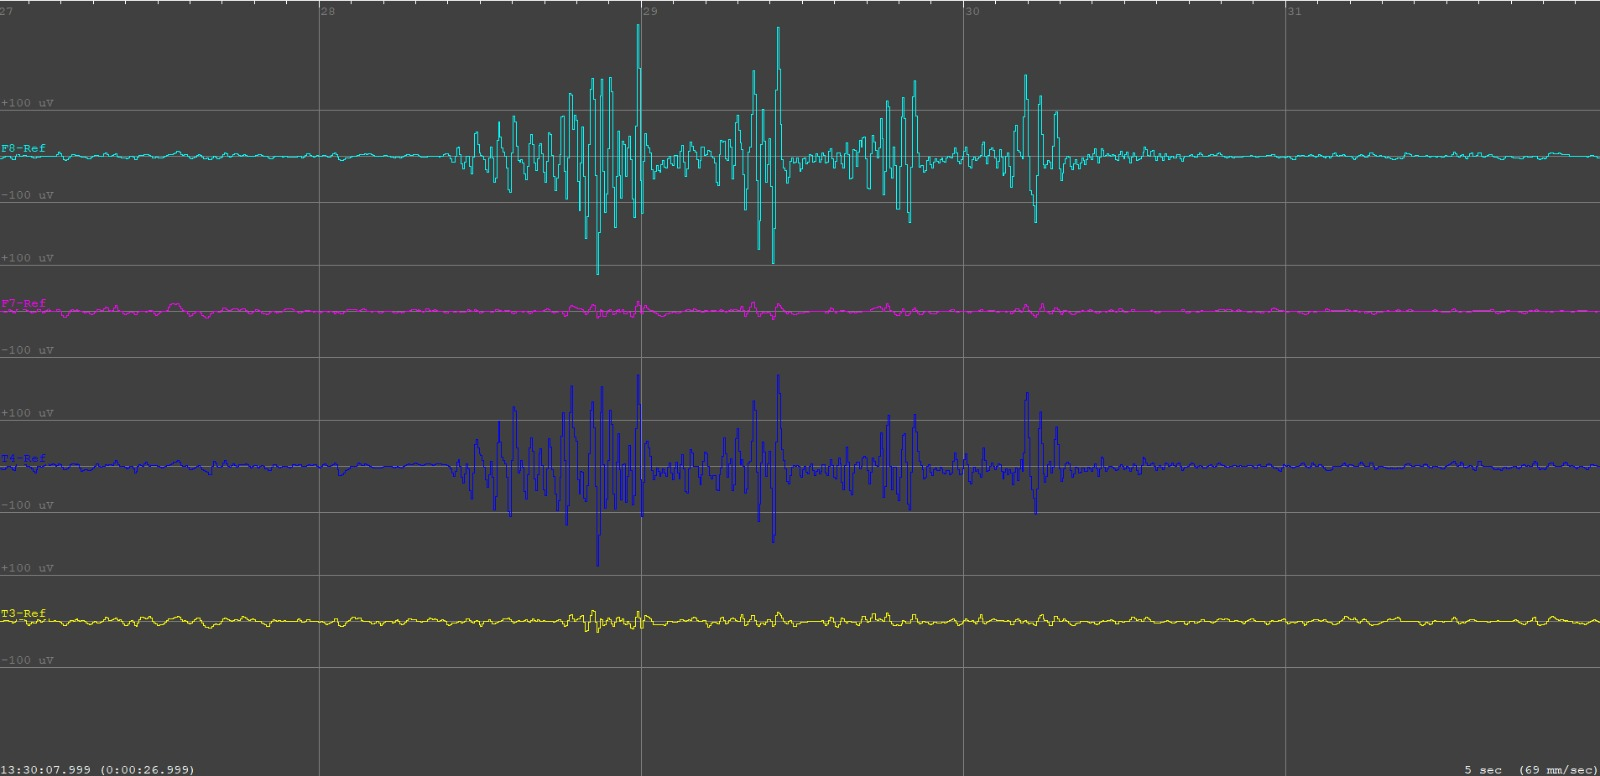
\includegraphics[width=0.90\textwidth]{Assets/signal_bruxism_r}
\caption{EEG signal at T3 and T4 during voluntary \textbf{right
bruxism}. T4 (right temporal) shows clearly higher amplitude
than T3 (left temporal), reflecting preferential activation
of the right temporalis muscle. The normalised asymmetry index
$\mathcal{A}_{T3,T4} > 0$ for this class. Comparing this
figure with Figure~\ref{fig:signal_bruxism_left} clearly
demonstrates the lateral asymmetry that the T3--T4 asymmetry
feature (Chapter~8) is designed to capture.}
\label{fig:signal_bruxism_right}
\end{figure}

%% ----------------------------------------------------------
\section{Data Directory Structure}
\label{sec:dc_structure}
%% ----------------------------------------------------------

The complete dataset is organised in a hierarchical directory
structure that the data loader (\code{loader.py}) traverses
automatically, auto-discovering any \code{Session*} folder so
that new sessions can be added with zero code changes. The
structure is as follows:

\begin{lstlisting}[language=bash, caption={Dataset directory
structure. Session1 and Session2 share one file-naming
convention; Session3 uses a second convention (GLENCH*,
BRUXES*) that the loader normalises to the same class labels.
Each session contributes exactly 5 selected recordings (one per
final class) for 15 \acrshort{edf} recordings in total; the
*03/*DOUBLE files (triple blink, bilateral bruxism/clinch) are
present on disk but excluded from the final 5-class dataset.},
label={lst:dir_structure}]
DATA/
|-- Session1/                  # Training data - Session 1
|   |-- Blink/
|   |   |-- BLINK01.edf       # Single blink recordings
|   |   |-- BLINK02.edf       # Double blink recordings
|   |   `-- BLINK03.edf       # (not used - triple blink dropped)
|   |-- Bruxissem/
|   |   |-- LEFT.edf          # Left bruxism recordings
|   |   `-- RIGHT.edf         # Right bruxism recordings
|   `-- Clinch/
|       |-- Bilateral/
|       |   `-- *.edf         # Bilateral clinch recordings
|       `-- Bileteral/        # Typo variant - also loaded
|           `-- *.edf
|-- Session2/                  # Training data - Session 2
|   |-- Blink/                # Same structure as Session1
|   |-- Bruxissem/
|   `-- Clinch/
|-- Session3/                  # Training data - Session 3
|   |-- Blink/
|   |   |-- BLINK01.edf
|   |   |-- BLINK02.edf
|   |   `-- BLINK03.edf       # (not used - triple blink dropped)
|   |-- Bruxissem/
|   |   |-- BRUXESLEFT.edf
|   |   |-- BRUXESRIGHT.edf
|   |   `-- BRUXESDOUBLE.edf  # (not used - bilateral, mislabel risk)
|   `-- Clinch/
|       |-- GLENCHLEFT.edf
|       |-- GLENCHRIGHT.edf
|       `-- GLENCHDOUBLE.edf  # (not used - bilateral, mislabel risk)
`-- Random/                    # Mixed-gesture validation set (see
                                # Section 6.6) - unsynchronised
                                # timestamps, not used for training
\end{lstlisting}

\subsection{Loader Design and Auto-Scanning}

The data loader (\code{loader.py}) was designed to automatically
discover and load all \acrshort{edf} files matching the expected
class patterns, without requiring manual file path specification.
The loader performs the following steps:

\begin{enumerate}[leftmargin=*]
    \item Scan the \code{DATA/} root directory for all
    sub-directories matching the pattern \code{Session*}, so
    that Session3 (and any future session) is picked up with no
    code changes.
    \item Within each session directory, search for
    \code{Blink/}, \code{Bruxissem/}, and \code{Clinch/}
    sub-directories.
    \item Within \code{Blink/}, match files named
    \code{BLINK01.edf} and \code{BLINK02.edf} and assign labels
    \code{single\_blink} and \code{double\_blink} respectively.
    \code{BLINK03.edf} (triple blink) is discovered but excluded
    at the label-mapping stage (Section~\ref{sec:dc_labels}).
    \item Within \code{Bruxissem/}, match files containing
    \code{LEFT} or \code{RIGHT} in their filename (covering both
    the \code{LEFT}/\code{RIGHT} convention of Session1/Session2
    and the \code{BRUXESLEFT}/\code{BRUXESRIGHT} convention of
    Session3). Files containing \code{DOUBLE} are discovered but
    excluded, since bilateral bruxism is not part of the final
    taxonomy.
    \item Within \code{Clinch/}, recursively search all
    sub-directories and filenames for \acrshort{edf} files and
    assign the \code{clinch} label, matching both the
    \code{Bilateral}/\code{Bileteral} sub-folder convention of
    Session1/Session2 and the \code{GLENCHLEFT}/\code{GLENCHRIGHT}
    filename convention of Session3. \code{GLENCHDOUBLE} files
    are discovered but excluded for the same reason as bilateral
    bruxism (Section~\ref{sec:dc_bug}).
    \item Return a list of \code{(filepath, label)} tuples
    covering all discovered, non-excluded files across all
    sessions.
\end{enumerate}

\subsection{Loader Bug: Silent Clinch Data Loss}
\label{sec:dc_bug}

During initial development, a critical bug was discovered in
the data loader that caused a meaningful fraction of clinch
training data to be silently discarded. The root cause was a
folder naming inconsistency: the recording software saved a
sub-session of clinch recordings into a folder named
\textbf{``Bileteral''} (a typographical error) rather than the
expected \textbf{``Bilateral''}. The original loader recognised
only the ``Bilateral'' spelling as a valid folder name, causing
the typo variant to be silently skipped.

\textbf{Impact:} At the time this bug was active (an earlier,
2-session development iteration of the pipeline, prior to the
current finalised 3-session/15-recording dataset described in
Section~\ref{sec:dc_stats}), the loader was silently dropping 2
clinch recordings, which meant the model was being trained on
1{,}002 clinch epochs instead of the correct 1{,}328 --- a loss
of 326 epochs (24.6\%). Since clinch is consistently the
highest-performing class, the impact on overall accuracy was
limited, but the silent nature of the failure is concerning: the
system gave no warning that data was being dropped, making the
bug difficult to diagnose. The same class of problem --- a
naming-convention mismatch silently dropping data --- reappeared
conceptually when Session3 was added with its \code{GLENCH*} /
\code{BRUXES*} naming convention, which is why the loader logic
above was generalised to handle multiple naming conventions per
class rather than patched for a single spelling variant. The bug
is fixed and does not affect the current dataset counts reported
in Section~\ref{sec:dc_stats}.

\textbf{Fix:} The loader was updated to perform
case-insensitive recursive scanning of all sub-directories under
\code{Clinch/}, accepting any folder name, and to match multiple
known filename conventions per class across sessions. A
validation report is now printed on startup listing the number
of \acrshort{edf} files discovered per class per session,
enabling quick visual verification that no files are being
missed or unexpectedly excluded.

%% ----------------------------------------------------------
\section{Dataset Statistics}
\label{sec:dc_stats}
%% ----------------------------------------------------------

\subsection{Overall Dataset Size}

Dataset statistics were computed by running the actual data
pipeline --- \code{loader.discover\_recordings} $\rightarrow$
\code{preprocessing.preprocess\_all\_dual} $\rightarrow$
\code{activity\_gate.gate\_mask} (gate fraction 0.5, the same
value used by \code{train\_hierarchical.py},
\code{train\_hybrid.py}, and \code{train\_dtw\_hybrid.py}) --- on
the current 15-recording, 3-session, 5-class dataset. This
supersedes any earlier (6-class, 2-session) figures that may
appear elsewhere in project notes. The activity gate is
\textbf{recording-relative}: for each recording, an epoch is
kept only if its \acrshort{rms} energy exceeds 50\% of that
same recording's own activity level, rather than a single fixed
threshold shared across all recordings.

Before activity gating (post crop/filter/reject, epochs still
include rest windows), the dataset totals 2{,}564 epochs; after
gating, 1{,}246 epochs are retained (48.6\% overall). Both
figures are broken down by session and class in
Table~\ref{tab:dataset_stats_before} and
Table~\ref{tab:dataset_stats_after}.

\begin{table}[htbp]
\centering
\caption{Epoch counts per session per class, \emph{before}
activity gating (post crop/filter/reject, includes rest
windows).}
\label{tab:dataset_stats_before}
\renewcommand{\arraystretch}{1.3}
\begin{tabular}{l c c c c c c}
\toprule
\textbf{Session} & \code{double\_} & \code{single\_} &
\code{clinch} & \code{bruxism\_} & \code{bruxism\_} &
\textbf{Total} \\
 & \code{blink} & \code{blink} & & \code{left} & \code{right} & \\
\midrule
Session1 & 258 & 199 & 187 & 137 & 137 & 918 \\
Session2 & 79  & 191 & 137 & 79  & 137 & 623 \\
Session3 & 199 & 199 & 166 & 199 & 260 & 1{,}023 \\
\midrule
\textbf{Total} & 536 & 589 & 490 & 415 & 534 & \textbf{2{,}564} \\
\bottomrule
\end{tabular}
\end{table}

\begin{table}[htbp]
\centering
\caption{Epoch counts per session per class, \emph{after}
activity gating (gate fraction 0.5, recording-relative) --- the
counts actually used for training and \acrshort{loso}
evaluation (Chapter~9).}
\label{tab:dataset_stats_after}
\renewcommand{\arraystretch}{1.3}
\begin{tabular}{l c c c c c c}
\toprule
\textbf{Session} & \code{double\_} & \code{single\_} &
\code{clinch} & \code{bruxism\_} & \code{bruxism\_} &
\textbf{Total} \\
 & \code{blink} & \code{blink} & & \code{left} & \code{right} & \\
\midrule
Session1 & 114 & 70 & 58 & 56  & 70  & 368 \\
Session2 & 53  & 98 & 58 & 61  & 99  & 369 \\
Session3 & 88  & 94 & 49 & 122 & 156 & 509 \\
\midrule
\textbf{Total} & 255 & 262 & 165 & 239 & 325 & \textbf{1{,}246} \\
\bottomrule
\end{tabular}
\end{table}

Table~\ref{tab:dataset_retention} summarises retention per class
--- the fraction of before-gate epochs that survive activity
gating.

\begin{table}[htbp]
\centering
\caption{Per-class retention after activity gating (frac = 0.5),
pooled across all three sessions.}
\label{tab:dataset_retention}
\renewcommand{\arraystretch}{1.3}
\begin{tabular}{l c c c}
\toprule
\textbf{Class} & \textbf{Before Gate} & \textbf{After Gate} &
\textbf{Retained} \\
\midrule
\code{double\_blink}  & 536   & 255   & 47.6\% \\
\code{single\_blink}  & 589   & 262   & 44.5\% \\
\code{clinch}         & 490   & 165   & 33.7\% \\
\code{bruxism\_left}  & 415   & 239   & 57.6\% \\
\code{bruxism\_right} & 534   & 325   & 60.9\% \\
\midrule
\textbf{Total} & \textbf{2{,}564} & \textbf{1{,}246} & \textbf{48.6\%} \\
\bottomrule
\end{tabular}
\end{table}

Unlike the flat, near-uniform retention rate observed under the
earlier 2-session/6-class taxonomy, retention here varies
substantially by class --- from 33.7\% (clinch) to 60.9\%
(bruxism\_right). This is a direct consequence of the gate being
\textbf{recording-relative}: because the threshold for each
recording is set from that recording's own activity level (its
90th-percentile \acrshort{rms}) rather than a single global
value, retention depends on how each individual recording's
active-to-rest ratio compares to its own peak activity, which in
turn depends heavily on per-recording duration and gesture rate.
Session2's recordings are noticeably shorter (roughly 80--200\,s)
than those of Session1 and Session3 (roughly 140--261\,s), which
is reflected in Session2's generally lower before-gate epoch
counts in Table~\ref{tab:dataset_stats_before}.

\subsection{Class Imbalance}

Table~\ref{tab:dataset_retention} shows the resulting class
imbalance in the final, gated dataset: \code{bruxism\_right}
(325 epochs) is now the largest class and \code{clinch} (165
epochs) the smallest --- a reversal of the earlier
(2-session/6-class) dataset, in which clinch was by far the
largest class. This reversal is driven entirely by clinch's low
retention rate (33.7\%, the lowest of the five classes): clinch
recordings produce a raw (before-gate) epoch count comparable to
the blink classes (490), but the smallest fraction of those
epochs clears its own recording's activity threshold. The exact
recording-level cause of this lower retention (e.g., gesture
duration, pacing, or amplitude profile within the clinch
recordings specifically) was not established in the reviewed
source material and would be worth a short follow-up check
before final submission. This imbalance is addressed during
training using \acrshort{smote}, applied only to the training
fold in each cross-validation split to avoid leakage (Chapter~9).

%% ----------------------------------------------------------
\section{Label Scheme Evolution: From 9 Cued Classes to 5 Robust Classes}
\label{sec:dc_labels}
%% ----------------------------------------------------------

The final 5-class scheme is the result of two rounds of taxonomy
simplification, both driven by diagnostic findings rather than
assumptions made in advance.

\subsection{Round 1: 5 Classes $\rightarrow$ 6 Classes (+3.0\%)}

In an early version of the pipeline, single blinks
(\code{BLINK01}) and multi-blink bursts were merged into a
single ``blink'' class, on the assumption that they could be
treated as one command. This produced a 5-class scheme:
\{single/triple blink, double blink, clinch, bruxism\_left,
bruxism\_right\}.

This merging proved to be a significant error. \code{BLINK01}
recordings are nominally single blinks, while \code{BLINK03}
recordings are triple blinks; merging them into one class
created a training set with contradictory examples --- some
epochs showing a single peak, others showing three peaks --- for
which the classifier could not learn a consistent decision
boundary. The fix was to split the blink recordings into three
independent classes --- \code{single\_blink}, \code{double\_blink},
and \code{triple\_blink} --- each sourced exclusively from its
corresponding recording file. This produced a 6-class scheme and
improved overall accuracy from 80.4\% to 83.4\% (+3.0\%), with
the largest gains in the blink and bruxism classes:

\begin{itemize}[leftmargin=*]
    \item single\_blink F1: $0.818 \rightarrow 0.885$ (+0.067)
    \item bruxism\_left F1: $0.609 \rightarrow 0.737$ (+0.128)
\end{itemize}

\subsection{Round 2: 6 Classes $\rightarrow$ 5 Classes (final)}

A second, later round of simplification dropped
\code{triple\_blink} and excluded bilateral bruxism (which had,
at one point, been mislabelled and folded into \code{clinch}, as
noted in Section~\ref{sec:dc_structure}). Two findings motivated
this:

\begin{enumerate}[leftmargin=*]
    \item \textbf{Triple blink craters the blink stage regardless
    of method}, to around 56\% accuracy, whichever sub-classifier
    is used: double and triple blinks are only 300--400\,ms apart
    and effectively merge into one another at this timing
    resolution, making the three-way blink distinction unreliable
    however it is approached.
    \item \textbf{The single-blink contamination finding}
    (Section~\ref{sec:dc_single_blink}) showed that a large
    fraction of ``single blink'' trials already resemble
    multi-blink bursts, which compounds the triple-blink boundary
    problem: with three overlapping blink classes, the
    single/double/triple decision boundaries become unreliable
    exactly where the data is noisiest.
\end{enumerate}

Dropping the two hardest, most ambiguous gesture variants ---
triple blink and bilateral bruxism --- in favour of five robust,
well-separated commands is treated in this project as a
legitimate engineering decision for a \emph{working} prosthetic
control scheme, rather than as a limitation to be apologised for:
a smaller command set that the classifier gets right consistently
is more useful than a larger one that it gets wrong
unpredictably. The final taxonomy is:

\begin{center}
\{\code{single\_blink}, \code{double\_blink}, \code{clinch},
\code{bruxism\_left}, \code{bruxism\_right}\}
\end{center}

%% ----------------------------------------------------------
\section{Mixed-Gesture Validation Data}
\label{sec:dc_devtest}
%% ----------------------------------------------------------

In addition to the three per-class training sessions, a
\textbf{Random/} recording was collected: a single continuous
\acrshort{edf} file containing all five gestures performed in
random order, intended as the cleanest possible real-world,
free-running validation --- closer to how the system is actually
used than the isolated, single-class training sessions. An
accompanying \code{markers.csv} logs the timestamp and class
label of each gesture as it was performed by the experimenter,
intended to allow precise epoch extraction aligned to the actual
gesture events.

\textbf{This validation attempt failed, and is documented here
rather than discarded, because the failure is instructive.} The
\acrshort{edf} recording and the \code{markers.csv} file were
produced on two separate, unsynchronised clocks (the EEG
amplifier's internal clock and the marker-logging application's
system clock), and no reliable order-based burst-alignment method
could recover a valid correspondence between them --- both
alignment approaches that were tried landed close to chance
level. This is a \textbf{data-acquisition limitation}, not a
model failure: the marker timestamps simply cannot be trusted to
line up with the recording. Consequently, the \code{Random/}
session was not used for either threshold tuning or final
evaluation; the honest evaluation protocol used throughout this
project is Leave-One-Session-Out over Session1/Session2/Session3
(Chapter~9), not a held-out mixed-gesture file.

The clear lesson carried forward into future work (Chapter~14)
is that event markers should be recorded directly on the EEG
acquisition device itself, on the same clock as the signal,
rather than in a separate application on a separate clock.

%% ----------------------------------------------------------
\section{Chapter Summary}
\label{sec:dc_summary}
%% ----------------------------------------------------------

This chapter described the complete data collection methodology
for the \acrshort{bci} dataset. Recording was originally
protocolled around nine voluntary \acrshort{eeg} artifact gesture
classes, later narrowed to the five that make up the final,
deployed command set --- single blink, double blink, jaw clinch,
left bruxism, and right bruxism --- across three independent
recording sessions (Session1, Session2, and Session3) separated
by at least 24 hours each, organised in a hierarchical directory
structure that the loader auto-discovers. Two file-naming
conventions were used across sessions
(\code{BLINK}/\code{LEFT,RIGHT}/\code{Bilateral} in Session1--2
versus \code{BLINK}/\code{BRUXES*}/\code{GLENCH*} in Session3),
reconciled by the loader, which selects exactly one recording per
session per final class --- 15 \acrshort{edf} recordings in
total. Running the full pipeline
(\code{loader.discover\_recordings} $\rightarrow$
\code{preprocessing.preprocess\_all\_dual} $\rightarrow$
\code{activity\_gate.gate\_mask}, gate fraction 0.5) on this
dataset yields 2{,}564 epochs before activity gating and
1{,}246 epochs after, with per-class retention varying from
33.7\% (clinch) to 60.9\% (bruxism\_right) due to the
recording-relative nature of the gate. An earlier data loader bug
that silently discarded 326 clinch epochs (24.6\%) during a
2-session development iteration, due to a folder-naming typo, was
identified and corrected and does not affect these figures. A
critical data quality finding --- that roughly 45\% of ``single
blink'' recordings actually contain multi-blink clusters --- was
discovered during later diagnostic work and directly motivates
the shape-based (\acrshort{dtw}) blink classification approach of
Chapter~9. The label taxonomy evolved twice: first from 5 to 6
classes (+3.0\% accuracy, separating contaminated blink labels),
then from 6 to 5 classes (dropping triple blink and bilateral
bruxism as unreliable, low-value command variants). A
mixed-gesture validation recording (\code{Random/}) was attempted
but could not be used due to unsynchronised timestamps between
the EEG device and the marker-logging application --- a
data-acquisition lesson carried forward to future work. The
following chapter describes in detail the signal processing
pipeline applied to the raw \acrshort{edf} recordings.